% ============================================================
% Multiprocessor Scheduling
% ============================================================

\section{Multiprocessor Scheduling}

%------------------------------------------------
\begin{frame}{Multiprocessor Scheduling (Advanced)}

\begin{itemize}
    \item Multiprocessor systems have become commonplace with the rise of
    multicore processors.

    \item Multiple CPUs do not automatically make a single-threaded
    application faster.

    \item Multithreaded applications can spread work across multiple CPUs.

    \item The operating system must decide how to schedule jobs across
    multiple processors.
\end{itemize}

\vspace{0.3cm}

\begin{block}{Key Question}
How should the OS schedule jobs on multiple CPUs? What new problems arise?
Do the same old techniques work, or are new ideas required?
\end{block}

\end{frame}

%------------------------------------------------
\begin{frame}{Multiprocessor Architecture}

\begin{columns}

\column{0.55\textwidth}

\begin{itemize}
    \item CPUs use small and fast hardware caches.

    \item Main memory is larger but slower.

    \item Frequently accessed data can be stored in the cache.

    \item Caches exploit:
    \begin{itemize}
        \item \textbf{Temporal locality}
        \item \textbf{Spatial locality}
    \end{itemize}
\end{itemize}

\column{0.40\textwidth}

\centering
\begin{figure}
    \centering
    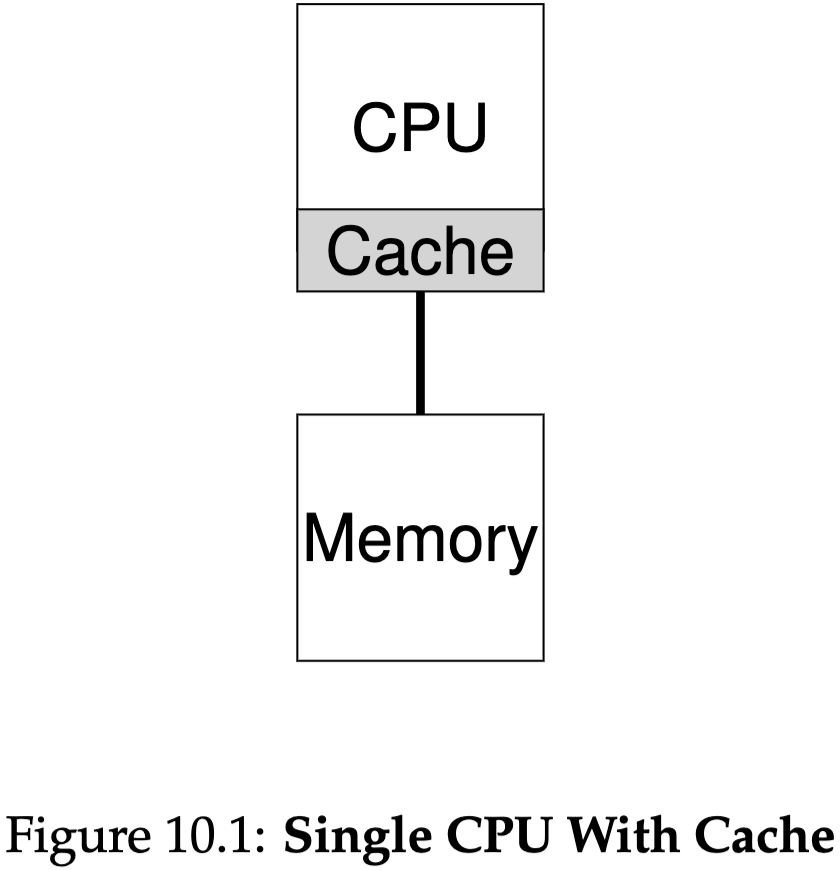
\includegraphics[width=1.1\linewidth]{figs/chapter-10/figure-10.1.png}
    \caption*{Source: chapter page 2.}
    \label{fig:figure-10.1}
\end{figure}

\end{columns}

\end{frame}

%------------------------------------------------
\begin{frame}{Multiprocessor Caches}

\begin{columns}

\column{0.54\textwidth}

\begin{itemize}
    \item Multiple CPUs may have private caches while sharing main memory.

    \item Different caches may contain different versions of the same
    memory location.

    \item This creates the \textbf{cache coherence} problem.

    \item Hardware must preserve the view of a single shared memory.
\end{itemize}

\column{0.42\textwidth}

\centering
\begin{figure}
    \centering
    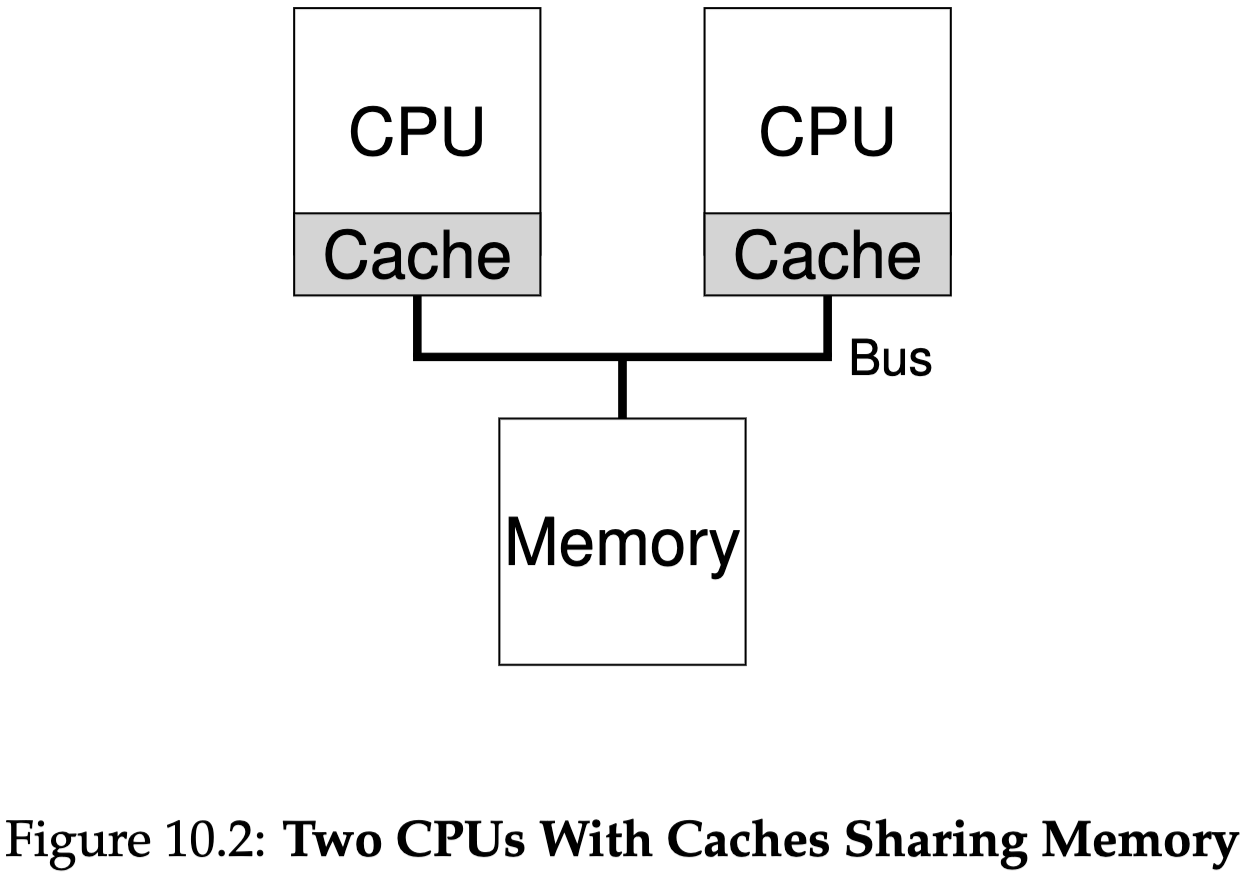
\includegraphics[width=1.1\linewidth]{figs/chapter-10/figure-10.2.png}
    \caption*{Source: chapter page 3.}
    \label{fig:figure-10.2}
\end{figure}

\end{columns}

\end{frame}

%------------------------------------------------
\begin{frame}{Cache Coherence}

\begin{itemize}
    \item Suppose CPU 1 reads a value $D$ from address $A$.

    \item CPU 1 modifies its cached value to $D'$.

    \item If the process later runs on CPU 2, CPU 2 may fetch the old
    value $D$ from memory.

    \item Hardware coherence mechanisms prevent this inconsistency.
\end{itemize}

\vspace{0.3cm}

\begin{block}{Bus Snooping}
Each cache monitors memory updates by observing the shared bus.

When a cache detects an update to one of its data items, it may:
\begin{itemize}
    \item invalidate its copy; or
    \item update its copy.
\end{itemize}
\end{block}

\end{frame}

%------------------------------------------------
\begin{frame}{Synchronization Is Still Necessary}

\begin{itemize}
    \item Cache coherence does \textbf{not} eliminate synchronization
    problems.

    \item Shared data structures may be accessed simultaneously by threads
    running on different CPUs.

    \item Mutual exclusion primitives, such as locks, are needed to
    guarantee correctness.

    \item Without synchronization, concurrent operations may corrupt
    shared data structures.
\end{itemize}

\end{frame}

%------------------------------------------------
\begin{frame}[fragile]{Example: Shared Linked List}

\begin{columns}

\column{0.51\textwidth}

\begin{lstlisting}[language=C,basicstyle=\ttfamily\scriptsize]
typedef struct __Node_t {
    int value;
    struct __Node_t *next;
} Node_t;

int List_Pop() {
    Node_t *tmp = head;
    int value = head->value;
    head = head->next;
    free(tmp);
    return value;
}
\end{lstlisting}

\column{0.45\textwidth}

\begin{itemize}
    \item Two threads may read the same \texttt{head}.

    \item Both may try to remove the same element.

    \item This may cause a double \texttt{free()}.

    \item The same data value may also be returned twice.

    \item Locking can make the operation execute correctly.
\end{itemize}

\end{columns}

% Figure 10.3
% Source: PDF page 5

\end{frame}

%------------------------------------------------
\begin{frame}{Cache Affinity}

\begin{itemize}
    \item A process builds state in a CPU's caches and TLBs.

    \item Running the process again on the same CPU may improve performance.

    \item Moving the process to another CPU requires its state to be
    reloaded.

    \item A multiprocessor scheduler should therefore consider
    \textbf{cache affinity}.
\end{itemize}

\vspace{0.3cm}

\begin{block}{Scheduling Goal}
Prefer keeping a process on the same CPU when possible.
\end{block}

\end{frame}

%------------------------------------------------
\begin{frame}{Single-Queue Multiprocessor Scheduling}

\begin{itemize}
    \item \textbf{SQMS}: Single-Queue Multiprocessor Scheduling.

    \item All jobs are placed into a single global scheduling queue.

    \item Existing single-CPU scheduling policies can be adapted relatively
    easily.
\end{itemize}

\vspace{0.3cm}

\begin{block}{Main Problems}
\begin{itemize}
    \item \textbf{Scalability}: access to the shared queue requires
    synchronization.

    \item \textbf{Cache affinity}: jobs may frequently migrate between CPUs.
\end{itemize}
\end{block}

% Suggested figure:
% First SQMS scheduling timeline
% Source: PDF page 6
% Suggested position: bottom of the slide

\end{frame}

%------------------------------------------------
\begin{frame}{SQMS and Cache Affinity}

\begin{itemize}
    \item With a global queue, jobs may move from one CPU to another.

    \item Frequent migration reduces the benefits of cached state.

    \item An affinity mechanism can keep most jobs on the same CPU.

    \item Some jobs may still migrate in order to balance the load.
\end{itemize}

\vspace{0.3cm}

% Suggested figure:
% Affinity-aware SQMS scheduling timeline
% Source: PDF page 7
% Suggested position: centered at the bottom

\centering
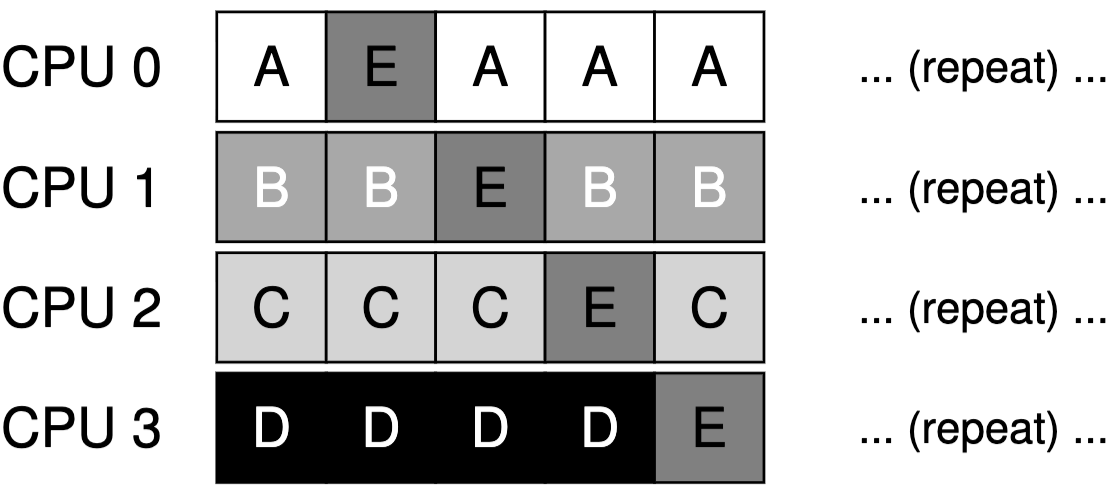
\includegraphics[width=0.70\linewidth]{figs/chapter-10/sqms-affinity.png}

\end{frame}

%------------------------------------------------
\begin{frame}{Multi-Queue Multiprocessor Scheduling}

\begin{itemize}
    \item \textbf{MQMS}: Multi-Queue Multiprocessor Scheduling.

    \item Each CPU has its own scheduling queue.

    \item Jobs are assigned to one queue when they enter the system.

    \item Each queue schedules its jobs essentially independently.
\end{itemize}

\vspace{0.3cm}

\begin{block}{Advantages}
\begin{itemize}
    \item Better scalability
    \item Reduced lock and cache contention
    \item Natural cache affinity
\end{itemize}
\end{block}

% Suggested figure:
% Two-CPU MQMS queues and round-robin timeline
% Source: PDF pages 7--8

\end{frame}

%------------------------------------------------
\begin{frame}{Load Imbalance}

\begin{itemize}
    \item Independent queues may develop different workloads.

    \item One CPU may have several runnable jobs while another CPU has
    fewer jobs.

    \item A CPU may even become completely idle while another CPU still
    has runnable jobs.
\end{itemize}

\vspace{0.3cm}

\begin{block}{Key Question}
How should a multi-queue multiprocessor scheduler handle load imbalance?
\end{block}

% Suggested figure:
% Load imbalance timelines
% Source: PDF page 8
% Suggested position: bottom of the slide

\end{frame}

%------------------------------------------------
\begin{frame}{Job Migration}

\begin{itemize}
    \item Load imbalance can be addressed by moving jobs between CPUs.

    \item This technique is called \textbf{migration}.

    \item If one CPU is idle, a job can be migrated from a busy CPU.

    \item In more complex situations, continuous migration of jobs may
    be needed to maintain balance.
\end{itemize}

% Suggested figure:
% Continuous migration timeline
% Source: PDF page 9
% Suggested position: bottom of the slide

\end{frame}

%------------------------------------------------
\begin{frame}{Work Stealing}

\begin{itemize}
    \item A queue with few jobs occasionally examines another queue.

    \item If the target queue is significantly more loaded, the source
    queue ``steals'' one or more jobs.

    \item This can improve load balance.
\end{itemize}

\vspace{0.3cm}

\begin{alertblock}{Trade-off}
Checking other queues too frequently increases overhead and hurts
scalability.

Checking too infrequently may result in severe load imbalance.
\end{alertblock}

\end{frame}

%------------------------------------------------
\begin{frame}{SQMS vs. MQMS}

\begin{center}
\begin{tabular}{lll}
\hline
 & \textbf{SQMS} & \textbf{MQMS} \\
\hline
Queues
    & Single global queue
    & Multiple queues \\

Scalability
    & More difficult
    & Better \\

Cache affinity
    & More difficult
    & Natural \\

Load balance
    & Easier
    & More difficult \\

Synchronization
    & Higher contention
    & Lower contention \\
\hline
\end{tabular}
\end{center}

\end{frame}

%------------------------------------------------
\begin{frame}{Summary}

\begin{itemize}
    \item Multiprocessor scheduling introduces new challenges beyond
    single-CPU scheduling.

    \item Cache coherence helps maintain a consistent view of shared memory.

    \item Synchronization is still required when accessing shared data.

    \item Cache affinity favors keeping processes on the same CPU.

    \item SQMS is straightforward but faces scalability and affinity
    problems.

    \item MQMS scales better but introduces load imbalance.

    \item Migration and work stealing can help balance CPU workloads.
\end{itemize}

\end{frame}